\chapter{周波数解析}
\section{\kadaiba}\label{sec:\kadaiba}
\purpose
\matlab を用いて周波数解析を行う.我々が普段見る「波形」は時間軸を横,振幅を縦にしたグラフである.
このグラフからわかるのは時刻に対しての振幅だ.ただし波形の分析はそれだけでは不十分である.
波形というのはフーリエ級数展開の理論により,いかなる波形も\eqref{equ:フーリエ級数展開}の\(N=\infty\)で表せる.
波形に対してフーリエ変換を行うと「周波数に対する振幅」を得ることができる.矩形波\eqref{equ:矩形波}の振幅と周波数をグラフに描画したものを振幅スペクトルと呼ぶ.(\ref{fig:周波数解析})\par
今回の実験では,純音と矩形波に対して周波数解析を行う.
純音では解析結果より純音の周波数をより多く含んでいるか確認する.
また矩形波では高調波の存在を確認し,振幅が\eqref{equ:矩形波}通りになっているか確かめる.
\begin{figure}[H]
    \centering
    \begin{minipage}{.4\textwidth}
    \renewcommand{\arraystretch}{1.5}
    \centering
    \begin{tabular}[c]{r|cc}
        \multicolumn{1}{c}{正弦波}   & 振幅                                                            & 周波数                                                             \\
        \hline
        \(2\sin(t)\)              & \tikz[remember picture,baseline=(A.base)]{\node(A){\(2\)}}    & \tikz[remember picture,baseline=(D.base)]{\node(D){\(1/2\pi\)}} \\
        \(-\sin (2t)\)            & \(-1\)                                                        & \(1/\pi\)                                                       \\
        \(\frac{2}{3}\sin (3t)\)  & \(2/3\)                                                       & \(3/2\pi\)                                                      \\
        \(-\frac{1}{2}\sin (4t)\) & \tikz[remember picture,baseline=(C.base)]{\node(C){\(-1/2\)}} & \tikz[remember picture,baseline=(B.base)]{\node(B){\(2/\pi\)}}  \\
        \multicolumn{3}{c}{{\LARGE\vdots}}
    \end{tabular}
    \begin{tikzpicture}[remember picture,overlay]
        \node[inner sep=0.1mm,fit={(A)(B)(C)(D)},draw,rounded corners,draw=blue](warp){};
    \end{tikzpicture}
    \begin{align*}
        f(t) & =\sum_{k=1}^{N}\frac{1}{2k-1}\sin\big(2\pi(2s-1)ft\big)\tag*{(\ref{equ:矩形波})}
    \end{align*}
\end{minipage}
\begin{minipage}{.4\textwidth}
    \centering
    \begin{tikzpicture}[remember picture]
        \node[left] at(0,0){O};
        \draw[very thick,-Stealth](0,0)--(5,0)node[midway,fill=white]{\scriptsize 周波数};
        \draw[very thick,-Stealth](0,-1.6)--(0,4.1)node[left]at($(0,0)!0.5!(0,4.1)$){\scriptsize \rotatebox{90}{振幅}};
        \foreach \u \v in {0.4/3,0.8/-1.5,1.2/1,1.6/-0.75}
        \draw[thick,blue](\u,0)--(\u,\v);
        \foreach \u \v \z in {0.4/{\(1/2\pi\)}/below,0.8/{\(1/\pi\)}/above,1.2/{\(3/2\pi\)}/below,1.6/{\(2/\pi\)}/above}
        \node[\z] at(\u,0){\tiny\v};
        \coordinate (O) at (0,0);
        \foreach \u \v \z \w in {0.4/3/a/{\(2\)},0.8/-1.5/b/{\(-1\)},1.2/1/c/{\(2/3\)},1.6/-0.75/d/{\(-1/2\)}} {
        \coordinate (\z) at (\u,\v);
        \draw[dotted,thin](\z)--(O |- \z)node[left]{\tiny\w};
        }
    \end{tikzpicture}
    \begin{tikzpicture}[remember picture,overlay]
        \draw[-latex,very thick,dashed]($(warp.south east)!0.5!(warp.north east)$)--($(O)+(-0.5cm,0)$);
    \end{tikzpicture}
\end{minipage}
    \caption{周波数解析}
    \label{fig:周波数解析}
\end{figure}
\method
\paragraph{高速フーリエ変換の実装}
\matlab では高速フーリエ変換をする関数(\texttt{fft})がある.
ただし,\texttt{fft}関数の仕様上いくつかの注意が必要である.データ列\texttt{y}に対して振幅スペクトルを取得する手順は以下の通りである.(\ref{src:振幅スペクトルの取得})
\begin{enumerate}
    \item 高速フーリエ変換を行う.\\
          \texttt{fft}関数は出力として,サンプリング周波数\texttt{Fs}に対して,\(\big[\textrm{\texttt{-Fs/2}},\textrm{\texttt{Fs/2}}\big]\)範囲の周波数に対する振幅のデータを得る.
    \item 出力データ列\texttt{fft(y)}のデータを整列させる.\\
          \texttt{fft}関数の出力は,正のデータ・負のデータ(左右)が入れ替わった状態で出力される.(\ref{fig:fft直後のデータ}\ -\ \ref{fig:fftshift後のデータ(グラフ)})
    \item これまでの過程で出力されるデータは複素数データである.絶対値を取るために\texttt{abs}関数を用いる.(\ref{fig:absを適用した後のデータ})
    \item グラフとして描画するために,周波数軸を作成する.(\ref{src:振幅スペクトルの取得})
\end{enumerate}
\begin{figure}[h]
    \centering
    \begin{minipage}[b]{.48\textwidth}
        \centering
        \begin{tikzpicture}
    \fill[fill=blue,opacity=0.1]($(.9\textwidth,0.5)!0.5!(0,0.5)$)rectangle(.9\textwidth,0);
    \fill[fill=red,opacity=0.1](0,0)rectangle($(.9\textwidth,0.5)!0.5!(0,0.5)$);
    \draw[thick](0,0)--(0.9\textwidth,0)--(0.9\textwidth,0.5)--(0,0.5)--cycle;
    \node[below] at (0,0)(a){\tiny\texttt{1}};
    \node[above] at (0,0.5){\tiny\texttt{0}};
    \node[above left] at ($(.9\textwidth,0.5)!0.5!(0,0.5)$){\tiny\texttt{Fs/2}};
    \node[above right] at ($(.9\textwidth,0.5)!0.5!(0,0.5)$){\tiny\texttt{-Fs/2}};
    \node[above] at (.9\textwidth,0.5){\tiny\texttt{-1/Fs}};
    \node[below] at (0.9\textwidth,0)(b){\tiny\texttt{Fs}};
    \draw[latex-latex](a)--(b)node[midway,below]{\tiny\texttt{index}};
    \coordinate (C) at ($(0.9\textwidth,0)!0.5!(0,0)$);
    \draw[thick](C)--($(C)+(0,1.5mm)$);
    \coordinate (c) at ($(0.9\textwidth,0.5)!0.5!(0,0.5)$);
    \draw[thick](c)--($(c)+(0,-1.5mm)$);
    \node at($(C)!0.5!(0,5mm)$){\tiny 正のデータ};
    \node at($(c)!0.5!(0.9\textwidth,0mm)$){\tiny 負のデータ};
\end{tikzpicture}
        \caption{\texttt{fft}直後の出力データ}
        \label{fig:fft直後のデータ}
    \end{minipage}
    \begin{minipage}[b]{.48\textwidth}
        \centering
        \begin{tikzpicture}
    \fill[fill=red,opacity=0.1]($(.9\textwidth,0.5)!0.5!(0,0.5)$)rectangle(.9\textwidth,0);
    \fill[fill=blue,opacity=0.1](0,0)rectangle($(.9\textwidth,0.5)!0.5!(0,0.5)$);
    \draw[thick](0,0)--(0.9\textwidth,0)--(0.9\textwidth,0.5)--(0,0.5)--cycle;
    \node[below] at (0,0)(a){\tiny\texttt{1}};
    \node[above] at (0,0.5){\tiny\texttt{-Fs/2}};
    \node[above left] at ($(.9\textwidth,0.5)!0.5!(0,0.5)$){\tiny\texttt{-1/Fs}};
    \node[above right] at ($(.9\textwidth,0.5)!0.5!(0,0.5)$){\tiny\texttt{0}};
    \node[above] at (.9\textwidth,0.5){\tiny\texttt{Fs/2}};
    \node[below] at (0.9\textwidth,0)(b){\tiny\texttt{Fs}};
    \draw[latex-latex](a)--(b)node[midway,below]{\tiny\texttt{index}};
    \coordinate (C) at ($(0.9\textwidth,0)!0.5!(0,0)$);
    \draw[thick](C)--($(C)+(0,1.5mm)$);
    \coordinate (c) at ($(0.9\textwidth,0.5)!0.5!(0,0.5)$);
    \draw[thick](c)--($(c)+(0,-1.5mm)$);
    \node at($(C)!0.5!(0,5mm)$){\tiny 負のデータ};
    \node at($(c)!0.5!(0.9\textwidth,0mm)$){\tiny 正のデータ};
\end{tikzpicture}
        \caption{\texttt{fftshift}後の出力データ}
        \label{fig:fftshift後のデータ}
    \end{minipage}
    \begin{minipage}[b]{.48\textwidth}
        \centering
        \begin{tikzpicture}
    \node(fig){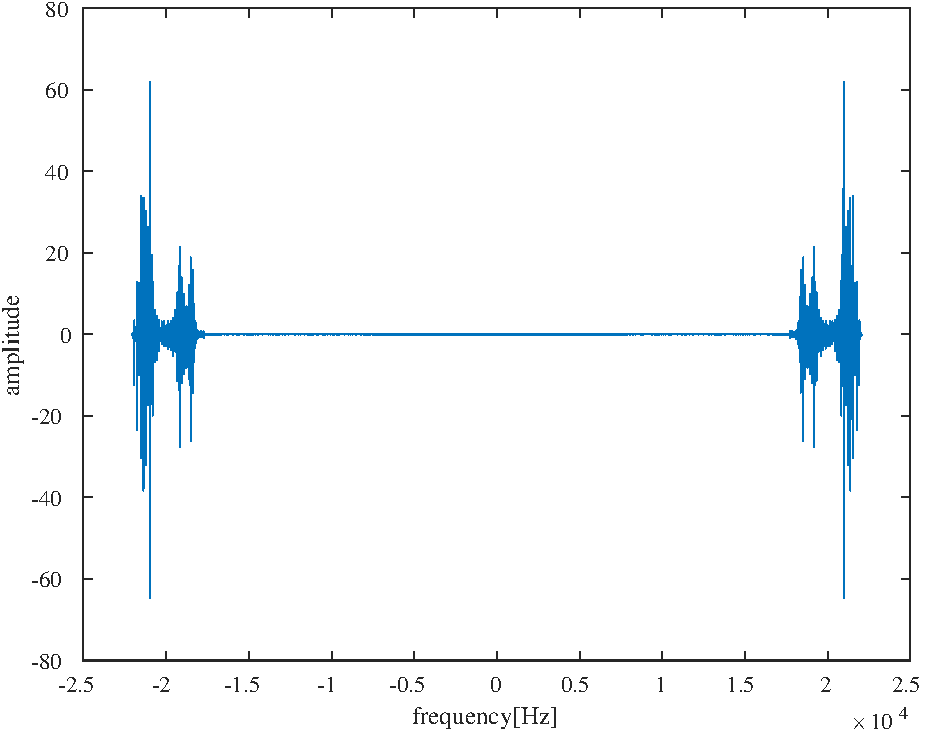
\includegraphics[keepaspectratio,width=.9\textwidth]{Figures/fft_fft.pdf}};
    \coordinate (figsouth) at (fig.south);
    \coordinate (figscenter) at ($(figsouth)+(2.75mm,7.1mm)$);
    \coordinate (figncenter) at ($(figscenter)+(0,5.48cm)$);
    \coordinate (figsleft) at ($(figscenter)+(-3.47cm,0)$);
    \coordinate (figsright) at ($(figscenter)+(3.47cm,0)$);
    \fill[fill=red,opacity=0.1](figsleft)--(figsleft |- figncenter)--(figncenter)--(figscenter)--cycle;
    \fill[fill=blue,opacity=0.1](figsright)--(figsright |- figncenter)--(figncenter)--(figscenter)--cycle;
    \coordinate (L) at($(figncenter)!0.5!(figsleft)+(0,1cm)$);
    \coordinate (R) at($(figncenter)!0.5!(figsright)+(0,1cm)$);
    \draw[very thick,dashed,latex-latex](L)to[bend left=40](R);
\end{tikzpicture}
        \caption{\texttt{fft}直後の出力データ(グラフ)}
        \label{fig:fft直後のデータ(グラフ)}
    \end{minipage}
    \begin{minipage}[b]{.48\textwidth}
        \centering
        \begin{tikzpicture}
    \node(fig){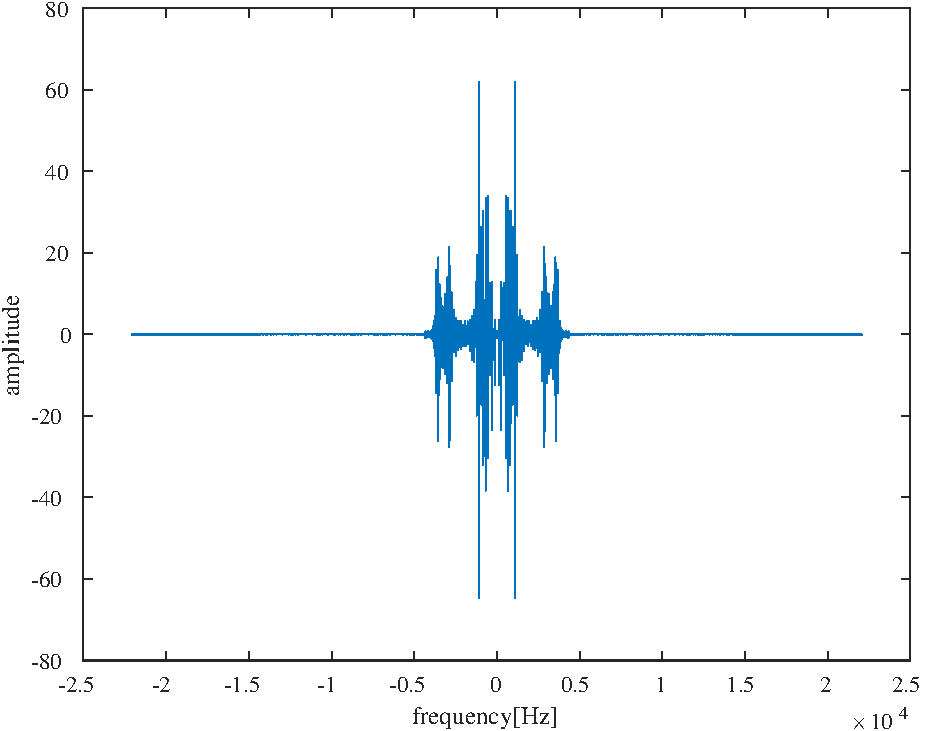
\includegraphics[keepaspectratio,width=.9\textwidth]{Figures/fft_fftshift.pdf}};
    \coordinate (figsouth) at (fig.south);
    \coordinate (figscenter) at ($(figsouth)+(2.75mm,7.1mm)$);
    \coordinate (figncenter) at ($(figscenter)+(0,5.48cm)$);
    \coordinate (figsleft) at ($(figscenter)+(-3.47cm,0)$);
    \coordinate (figsright) at ($(figscenter)+(3.47cm,0)$);
    \fill[fill=blue,opacity=0.1](figsleft)--(figsleft |- figncenter)--(figncenter)--(figscenter)--cycle;
    \fill[fill=red,opacity=0.1](figsright)--(figsright |- figncenter)--(figncenter)--(figscenter)--cycle;
\end{tikzpicture}
        \caption{\texttt{fftshift}後の出力データ(グラフ)}
        \label{fig:fftshift後のデータ(グラフ)}
    \end{minipage}\\
    \dotfill\\
    \begin{minipage}[b]{.48\textwidth}
        \centering
        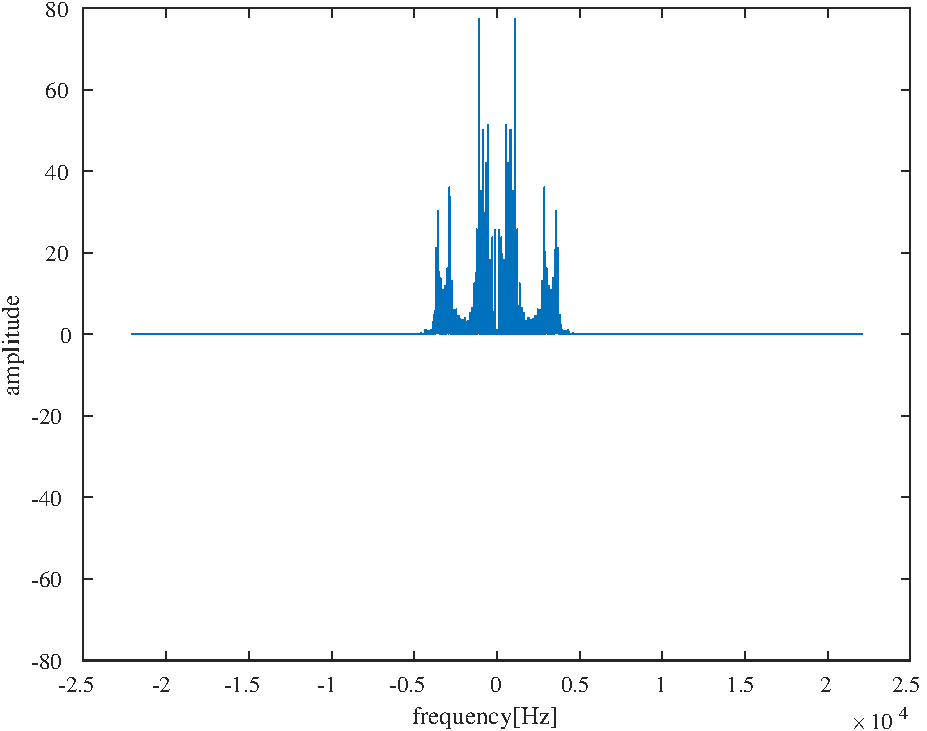
\includegraphics[keepaspectratio,width=.9\textwidth]{Figures/fft_abs.pdf}
        \caption{\texttt{abs}を適用した後のデータ(グラフ)}
        \label{fig:absを適用した後のデータ}
    \end{minipage}
    \begin{minipage}[b]{.48\textwidth}
        \centering
        \begin{lstlisting}[caption={振幅スペクトルの取得},label={src:振幅スペクトルの取得},xleftmargin={.5cm}]
y; % データ列
y_fft = fft(y); % 高速フーリエ変換
y_fftshift = fftshift(y_fft); % 左右交換
y_abs = fft_y; % 絶対値
ln = length(y_abs);
% 周波数テーブルの作成
freq = [-Fs/2 : Fs/ln : Fs/2 - Fs/ln];
plot(freq, y_abs); % グラフ描画
\end{lstlisting}
        \begin{flushleft}
            周波数テーブルの作成について,得られたデータ数\texttt{ln}に対して,
            周波数テーブルの長さ\texttt{Fs}に収める必要があるので,ステップ幅\texttt{Fs/ln}となる\texttt{-Fs/2}から\texttt{Fs/2}の配列を作成する.
        \end{flushleft}
    \end{minipage}
\end{figure}
\paragraph{実験の内容}今回の実験では,純音と矩形波の周波数解析を行う.サンプリング周波数を\(\textrm{\texttt{Fs}}=8192\textrm{Hz}\)と設定する.
\begin{figure}[H]
    \begin{minipage}[c]{.55\textwidth}
        \begin{itemize}
            \item[\textbf{純音}] \(440\textrm{Hz}\)の純音で実験する.
            \item 純音から\(1024\)点取り出す.\\
                  データ列の先頭から\(1024\)個のデータを選択する方法で行う.
            \item 振幅スペクトルを\(0\textrm{Hz}\)から\(1\textrm{kHz}\)まで描画する.
            \item \(440\textrm{Hz}\)にピークが来ているか確認する.
            \item[\textbf{矩形波}] \(128\)点値\(0\)が続き,\(128\)点値\(1\)が続く波形を\(4\)回繰り返す矩形波.(\ref{fig:作成した矩形波})
            \item 振幅スペクトルを\(0\textrm{Hz}\)から\(200\textrm{Hz}\)まで描画する.
            \item 高調波が発生しているか,その振幅が\eqref{equ:矩形波}通りになっているか確認する.
        \end{itemize}
        \srcref{sec:\kadaiba}{src:02_01_1}\(\underset{\Rightarrow\textrm{p.\pageref{src:02_01_2}}}{\textrm{\ref{src:02_01_2}}}\).
    \end{minipage}
    \begin{minipage}[c]{.4\textwidth}
        \centering
        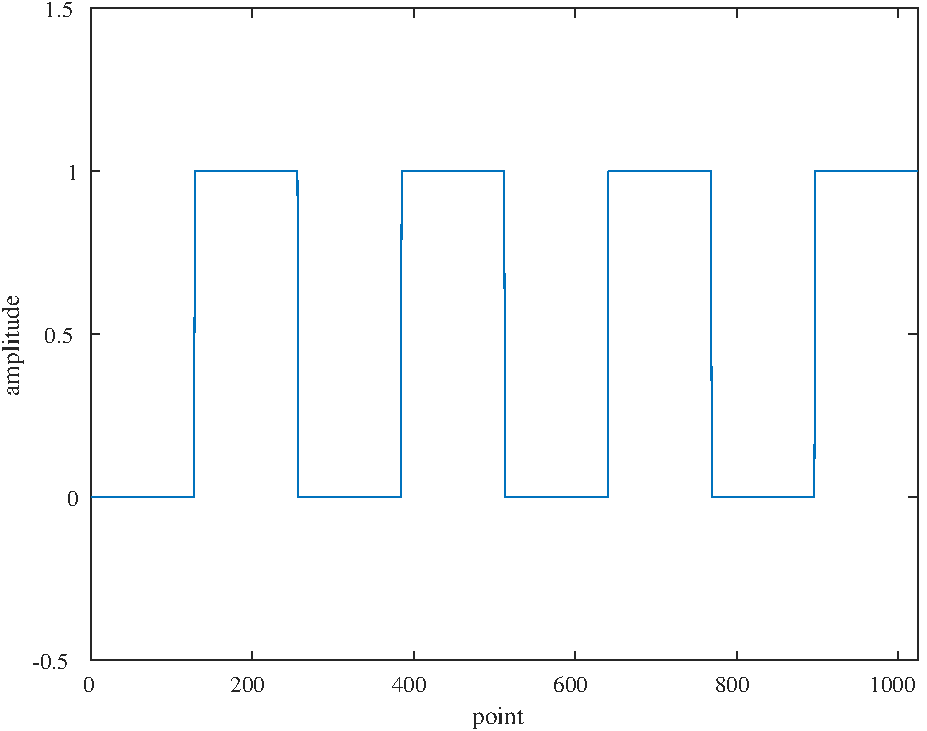
\includegraphics[keepaspectratio,width=\textwidth]{../../Figures/02_021.pdf}
        \caption{作成した矩形波}
        \label{fig:作成した矩形波}
    \end{minipage}
\end{figure}
\result
出力された結果に対して,特出する点の座標を表示させる.\ref{fig:\kadaiba_純音の振幅スペクトル}について,\(440\textrm{Hz}\)の軸に対して振幅が大きくあることがわかった.\par
\ref{fig:\kadaiba_矩形波の振幅スペクトル}については図中にある点の高調波が確認された.
\begin{figure}[h]
    \centering
    \begin{minipage}{.48\textwidth}
        \centering
        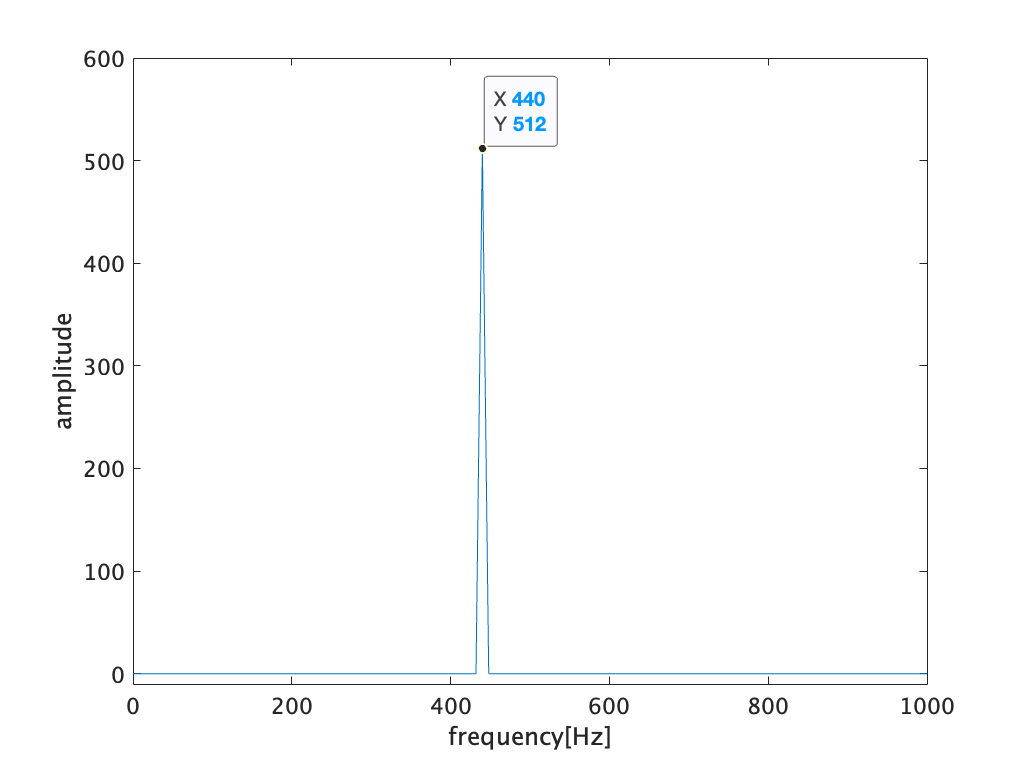
\includegraphics[keepaspectratio,width=\textwidth]{../../Figures/02_01.png}
        \caption{純音の振幅スペクトル}
        \label{fig:\kadaiba_純音の振幅スペクトル}
    \end{minipage}
    \begin{minipage}{.48\textwidth}
        \centering
        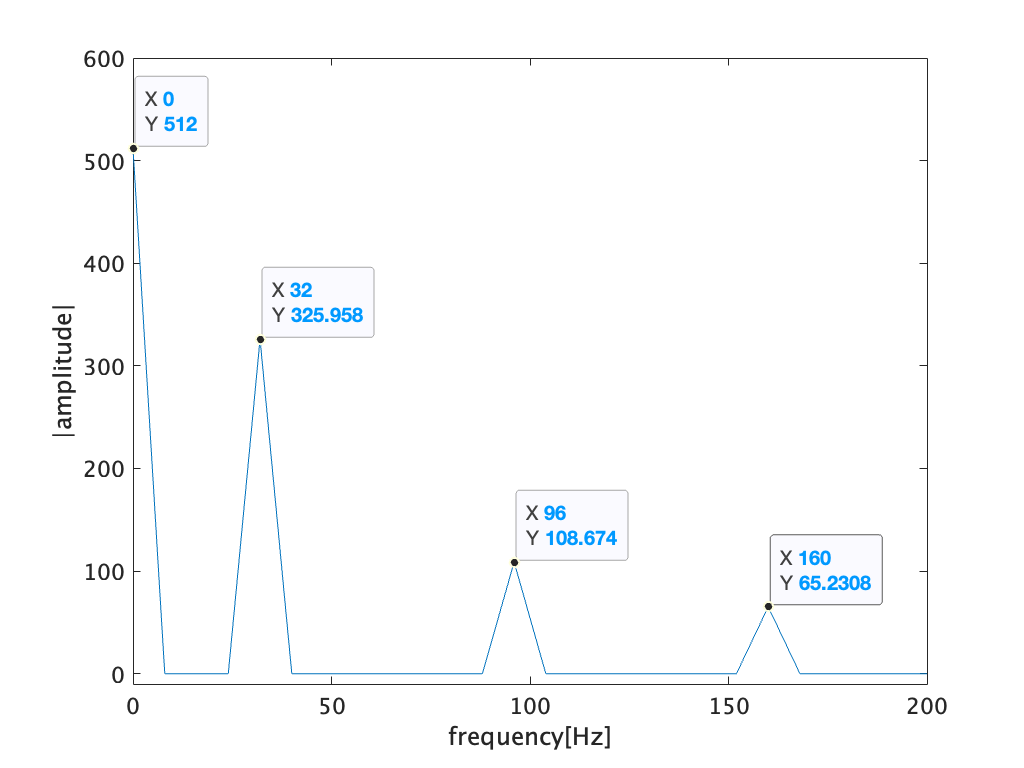
\includegraphics[keepaspectratio,width=\textwidth]{../../Figures/02_022.png}
        \caption{矩形波の振幅スペクトル}
        \label{fig:\kadaiba_矩形波の振幅スペクトル}
    \end{minipage}
\end{figure}
\consideration
\paragraph{純音}実験結果より,純音の周波数\(440\textrm{Hz}\)が一番多く,他の高調波はほとんど目立たない.
\paragraph{矩形波}\ref{fig:\kadaiba_矩形波の振幅スペクトル}より高調波の存在は確認できる.矩形波のフーリエ級数展開は\eqref{equ:矩形波}である.\(k=\{1,2,3,4\}\)のときの正弦波の式を\eqref{equ:矩形波具体例}に示す.
\begin{equation}
    \begin{aligned}
        \sin(2\pi(2-1)ft)            & =\sin(2\pi ft)             & (k=1) \\
        \frac{1}{3}\sin(2\pi(4-1)ft) & =\frac{1}{3}\sin(6\pi ft)  & (k=2) \\
        \frac{1}{5}\sin(2\pi(6-1)ft) & =\frac{1}{5}\sin(10\pi ft) & (k=3) \\
        \frac{1}{7}\sin(2\pi(8-1)ft) & =\frac{1}{7}\sin(14\pi ft) & (k=4) \\
    \end{aligned}\label{equ:矩形波具体例}
\end{equation}
これからわかるように,周波数が大きくなるにつれて振幅は小さくなることがわかる.これは\ref{fig:\kadaiba_矩形波の振幅スペクトル}と一致する.ただし,\eqref{equ:矩形波具体例}のように\(\frac{1}{3}, \frac{1}{5},\dots\)と変化しないのは\texttt{abs}関数の利用の際に振幅が変化するためと考えられるが(\ref{fig:absを適用した後のデータ}),詳しくは不明である.
また,\ref{fig:\kadaiba_矩形波の振幅スペクトル}と\eqref{equ:矩形波具体例}の周波数に関する関係も不明である.
\section{\kadaibb}\label{sec:\kadaibb}